\PassOptionsToPackage{unicode=true}{hyperref} % options for packages loaded elsewhere
\PassOptionsToPackage{hyphens}{url}
\PassOptionsToPackage{dvipsnames,svgnames*,x11names*}{xcolor}
%
\documentclass[ignorenonframetext,]{beamer}
\usepackage{pgfpages}
\setbeamertemplate{caption}[numbered]
\setbeamertemplate{caption label separator}{: }
\setbeamercolor{caption name}{fg=normal text.fg}
\beamertemplatenavigationsymbolsempty
% Prevent slide breaks in the middle of a paragraph:
\widowpenalties 1 10000
\raggedbottom
\setbeamertemplate{part page}{
\centering
\begin{beamercolorbox}[sep=16pt,center]{part title}
  \usebeamerfont{part title}\insertpart\par
\end{beamercolorbox}
}
\setbeamertemplate{section page}{
\centering
\begin{beamercolorbox}[sep=12pt,center]{part title}
  \usebeamerfont{section title}\insertsection\par
\end{beamercolorbox}
}
\setbeamertemplate{subsection page}{
\centering
\begin{beamercolorbox}[sep=8pt,center]{part title}
  \usebeamerfont{subsection title}\insertsubsection\par
\end{beamercolorbox}
}
\AtBeginPart{
  \frame{\partpage}
}
\AtBeginSection{
  \ifbibliography
  \else
    \frame{\sectionpage}
  \fi
}
\AtBeginSubsection{
  \frame{\subsectionpage}
}
\usepackage{lmodern}
\usepackage{amssymb,amsmath}
\usepackage{ifxetex,ifluatex}
\usepackage{fixltx2e} % provides \textsubscript
\ifnum 0\ifxetex 1\fi\ifluatex 1\fi=0 % if pdftex
  \usepackage[T1]{fontenc}
  \usepackage[utf8]{inputenc}
  \usepackage{textcomp} % provides euro and other symbols
\else % if luatex or xelatex
  \usepackage{unicode-math}
  \defaultfontfeatures{Ligatures=TeX,Scale=MatchLowercase}
\fi
% use upquote if available, for straight quotes in verbatim environments
\IfFileExists{upquote.sty}{\usepackage{upquote}}{}
% use microtype if available
\IfFileExists{microtype.sty}{%
\usepackage[]{microtype}
\UseMicrotypeSet[protrusion]{basicmath} % disable protrusion for tt fonts
}{}
\IfFileExists{parskip.sty}{%
\usepackage{parskip}
}{% else
\setlength{\parindent}{0pt}
\setlength{\parskip}{6pt plus 2pt minus 1pt}
}
\usepackage{xcolor}
\usepackage{hyperref}
\hypersetup{
            pdftitle={Introduction to R Programming},
            pdfauthor={Pedro Fonseca},
            colorlinks=true,
            linkcolor=Maroon,
            filecolor=Maroon,
            citecolor=Blue,
            urlcolor=blue,
            breaklinks=true}
\urlstyle{same}  % don't use monospace font for urls
\newif\ifbibliography
\usepackage{color}
\usepackage{fancyvrb}
\newcommand{\VerbBar}{|}
\newcommand{\VERB}{\Verb[commandchars=\\\{\}]}
\DefineVerbatimEnvironment{Highlighting}{Verbatim}{commandchars=\\\{\}}
% Add ',fontsize=\small' for more characters per line
\usepackage{framed}
\definecolor{shadecolor}{RGB}{248,248,248}
\newenvironment{Shaded}{\begin{snugshade}}{\end{snugshade}}
\newcommand{\AlertTok}[1]{\textcolor[rgb]{0.94,0.16,0.16}{#1}}
\newcommand{\AnnotationTok}[1]{\textcolor[rgb]{0.56,0.35,0.01}{\textbf{\textit{#1}}}}
\newcommand{\AttributeTok}[1]{\textcolor[rgb]{0.77,0.63,0.00}{#1}}
\newcommand{\BaseNTok}[1]{\textcolor[rgb]{0.00,0.00,0.81}{#1}}
\newcommand{\BuiltInTok}[1]{#1}
\newcommand{\CharTok}[1]{\textcolor[rgb]{0.31,0.60,0.02}{#1}}
\newcommand{\CommentTok}[1]{\textcolor[rgb]{0.56,0.35,0.01}{\textit{#1}}}
\newcommand{\CommentVarTok}[1]{\textcolor[rgb]{0.56,0.35,0.01}{\textbf{\textit{#1}}}}
\newcommand{\ConstantTok}[1]{\textcolor[rgb]{0.00,0.00,0.00}{#1}}
\newcommand{\ControlFlowTok}[1]{\textcolor[rgb]{0.13,0.29,0.53}{\textbf{#1}}}
\newcommand{\DataTypeTok}[1]{\textcolor[rgb]{0.13,0.29,0.53}{#1}}
\newcommand{\DecValTok}[1]{\textcolor[rgb]{0.00,0.00,0.81}{#1}}
\newcommand{\DocumentationTok}[1]{\textcolor[rgb]{0.56,0.35,0.01}{\textbf{\textit{#1}}}}
\newcommand{\ErrorTok}[1]{\textcolor[rgb]{0.64,0.00,0.00}{\textbf{#1}}}
\newcommand{\ExtensionTok}[1]{#1}
\newcommand{\FloatTok}[1]{\textcolor[rgb]{0.00,0.00,0.81}{#1}}
\newcommand{\FunctionTok}[1]{\textcolor[rgb]{0.00,0.00,0.00}{#1}}
\newcommand{\ImportTok}[1]{#1}
\newcommand{\InformationTok}[1]{\textcolor[rgb]{0.56,0.35,0.01}{\textbf{\textit{#1}}}}
\newcommand{\KeywordTok}[1]{\textcolor[rgb]{0.13,0.29,0.53}{\textbf{#1}}}
\newcommand{\NormalTok}[1]{#1}
\newcommand{\OperatorTok}[1]{\textcolor[rgb]{0.81,0.36,0.00}{\textbf{#1}}}
\newcommand{\OtherTok}[1]{\textcolor[rgb]{0.56,0.35,0.01}{#1}}
\newcommand{\PreprocessorTok}[1]{\textcolor[rgb]{0.56,0.35,0.01}{\textit{#1}}}
\newcommand{\RegionMarkerTok}[1]{#1}
\newcommand{\SpecialCharTok}[1]{\textcolor[rgb]{0.00,0.00,0.00}{#1}}
\newcommand{\SpecialStringTok}[1]{\textcolor[rgb]{0.31,0.60,0.02}{#1}}
\newcommand{\StringTok}[1]{\textcolor[rgb]{0.31,0.60,0.02}{#1}}
\newcommand{\VariableTok}[1]{\textcolor[rgb]{0.00,0.00,0.00}{#1}}
\newcommand{\VerbatimStringTok}[1]{\textcolor[rgb]{0.31,0.60,0.02}{#1}}
\newcommand{\WarningTok}[1]{\textcolor[rgb]{0.56,0.35,0.01}{\textbf{\textit{#1}}}}
\setlength{\emergencystretch}{3em}  % prevent overfull lines
\providecommand{\tightlist}{%
  \setlength{\itemsep}{0pt}\setlength{\parskip}{0pt}}
\setcounter{secnumdepth}{0}

% set default figure placement to htbp
\makeatletter
\def\fps@figure{htbp}
\makeatother


\setbeamerfont{caption name}{series=\bfseries}

\title{Introduction to R Programming}
\providecommand{\subtitle}[1]{}
\subtitle{Getting Started}
\author{Pedro Fonseca}
\date{08 May 2020}

\begin{document}
\frame{\titlepage}

\begin{frame}{R and Rstudio}
\protect\hypertarget{r-and-rstudio}{}

\begin{itemize}
\item
  R is a programming language and a free and open source software
  environment for statistical computing and graphics
\item
  RStudio is an integrated development environment (IDE) for R with
  free/open source and commercial versions
\item
  You can use R without using RStudio, but you can't use Rstudio without
  using R
\end{itemize}

\end{frame}

\begin{frame}{This is how R looks like}
\protect\hypertarget{this-is-how-r-looks-like}{}

\begin{figure}
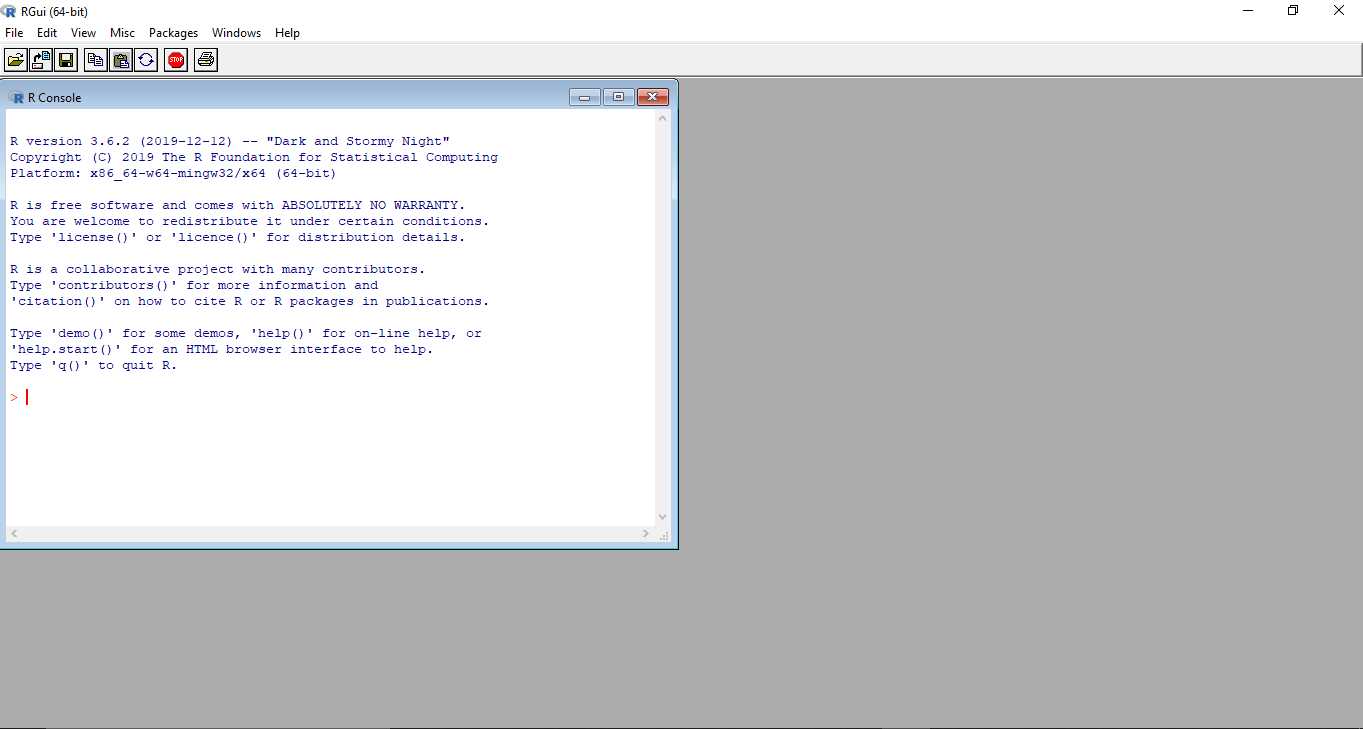
\includegraphics[scale = .3]{figures/Screenshot_1}
\caption{R on Windows}
\end{figure}

\end{frame}

\begin{frame}{This is how R looks like}
\protect\hypertarget{this-is-how-r-looks-like-1}{}

\begin{figure}
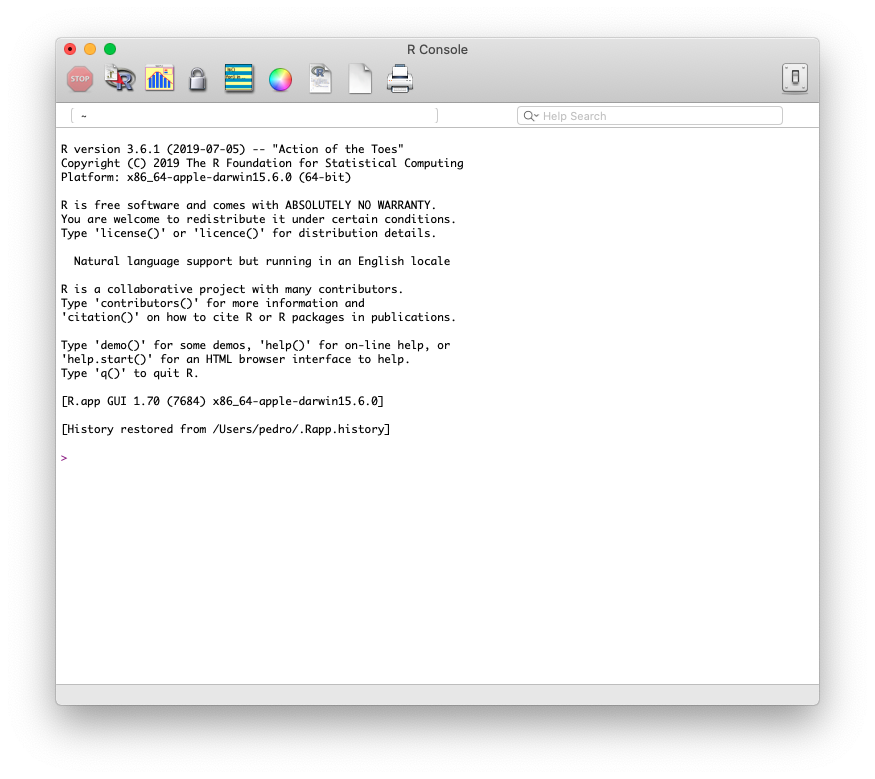
\includegraphics[scale = .26]{figures/r-mac}
\caption{R on macOS}
\end{figure}

\end{frame}

\begin{frame}{This is how R looks like}
\protect\hypertarget{this-is-how-r-looks-like-2}{}

\begin{figure}
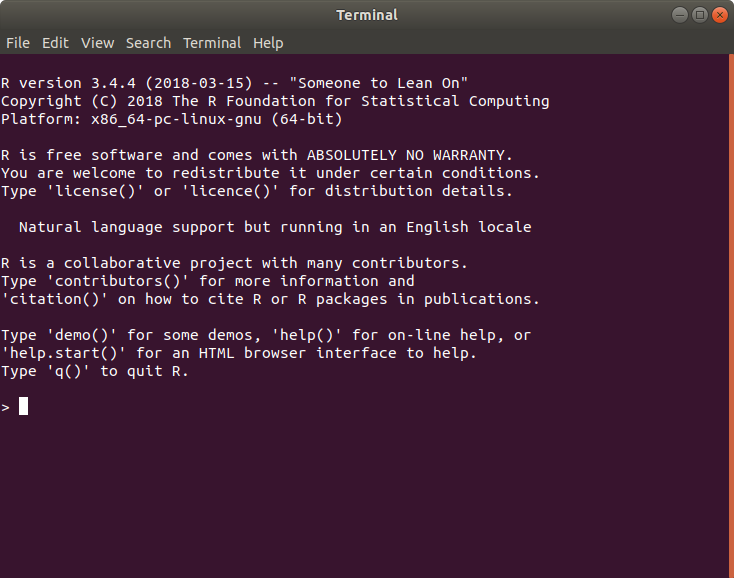
\includegraphics[scale = .3]{figures/r-linux}
\caption{R on Ubuntu}
\end{figure}

\end{frame}

\begin{frame}{This is how Rstudio looks like}
\protect\hypertarget{this-is-how-rstudio-looks-like}{}

Rstudio provides a user-friendly and interactive interface to R:

\begin{figure}[H]
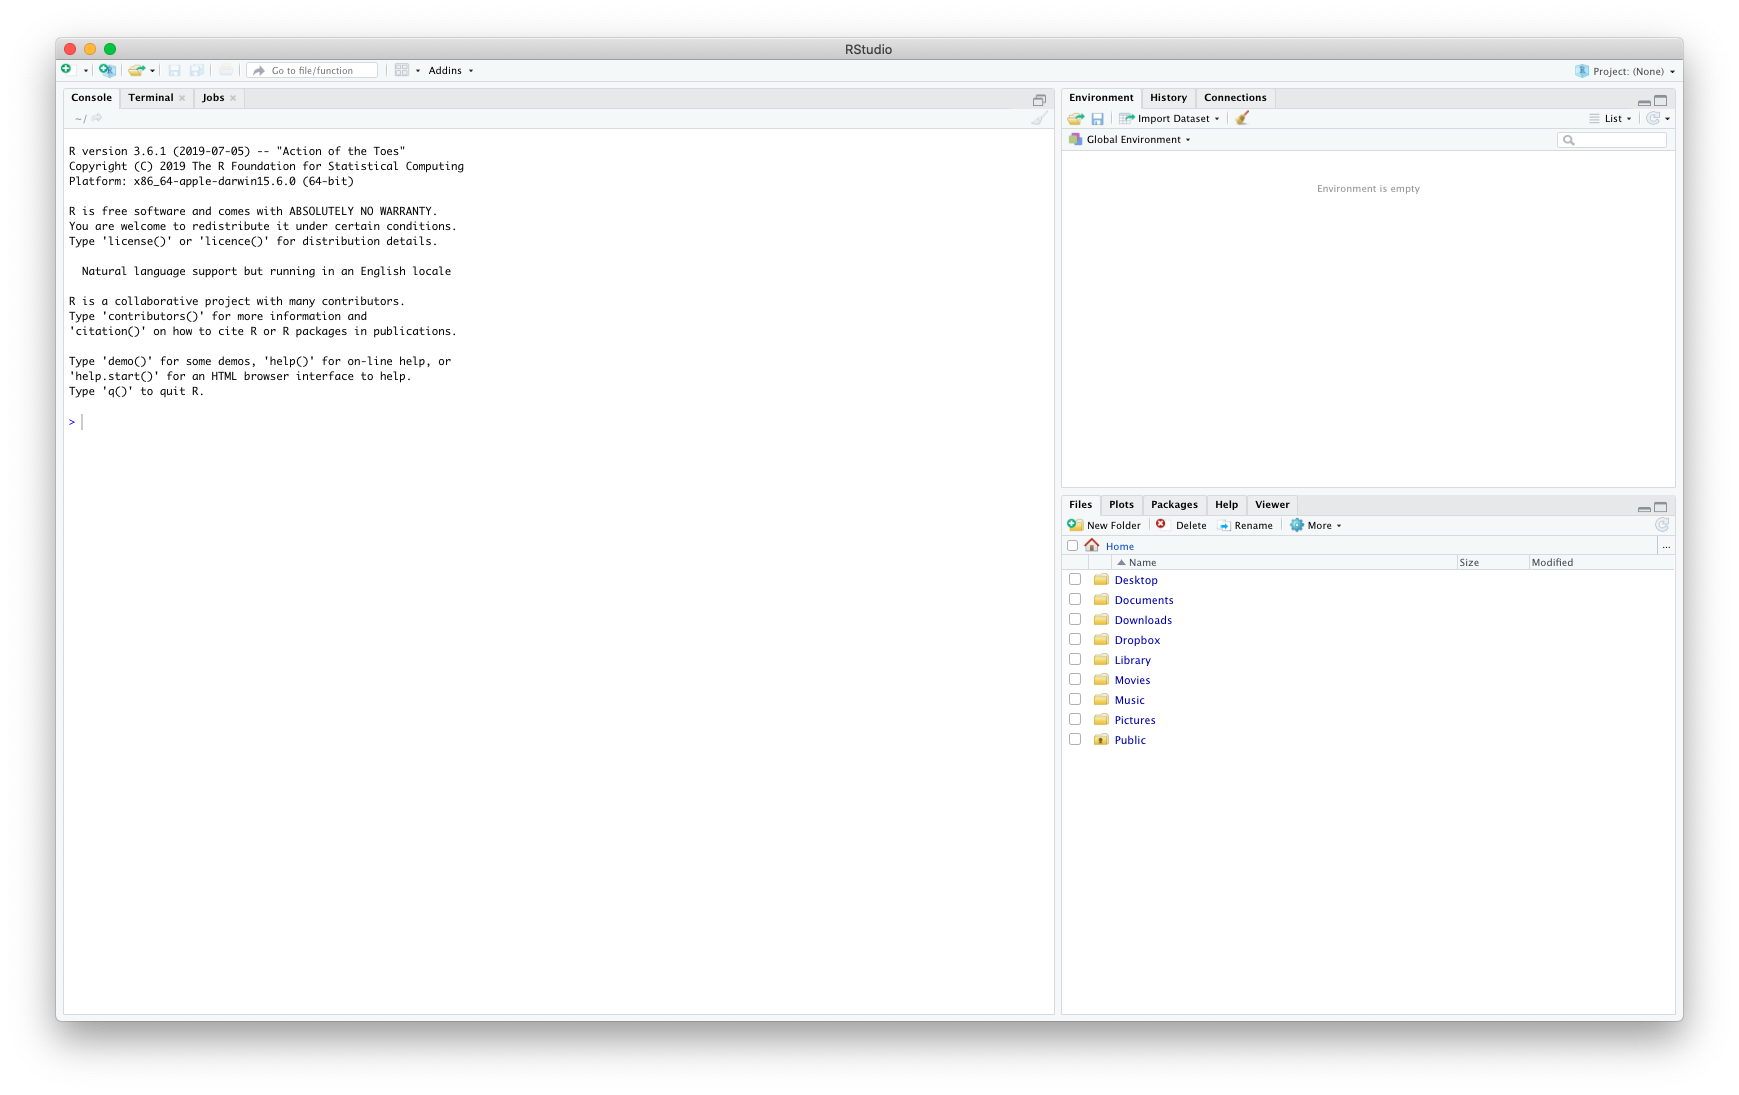
\includegraphics[scale = 0.15]{figures/Screenshot_mac}
\caption{RStudio}
\end{figure}

\end{frame}

\begin{frame}{The console}
\protect\hypertarget{the-console}{}

The pane on the left is the console. It can be used as a calculator:

\begin{figure}[H]
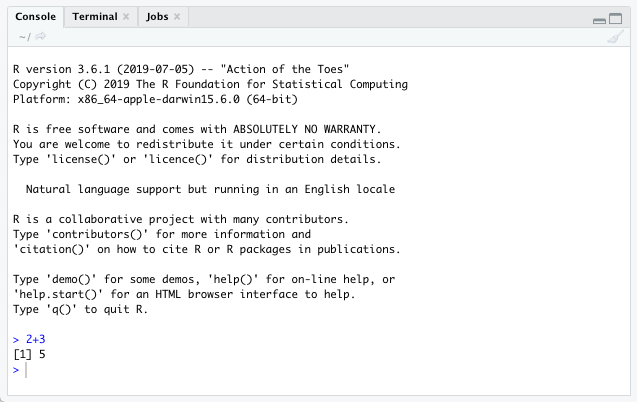
\includegraphics[scale = 0.35]{figures/calc}
\caption{R's console as a calculator}
\end{figure}

\end{frame}

\begin{frame}[fragile]{R as a calculator}
\protect\hypertarget{r-as-a-calculator}{}

\begin{Shaded}
\begin{Highlighting}[]
\DecValTok{2} \OperatorTok{+}\StringTok{ }\DecValTok{3} 
\end{Highlighting}
\end{Shaded}

\begin{verbatim}
## [1] 5
\end{verbatim}

\begin{Shaded}
\begin{Highlighting}[]
\DecValTok{3} \OperatorTok{*}\StringTok{ }\DecValTok{5}
\end{Highlighting}
\end{Shaded}

\begin{verbatim}
## [1] 15
\end{verbatim}

\begin{Shaded}
\begin{Highlighting}[]
\FloatTok{14.5} \OperatorTok{/}\StringTok{ }\DecValTok{6}
\end{Highlighting}
\end{Shaded}

\begin{verbatim}
## [1] 2.416667
\end{verbatim}

\begin{Shaded}
\begin{Highlighting}[]
\DecValTok{3} \OperatorTok{^}\StringTok{ }\DecValTok{2}
\end{Highlighting}
\end{Shaded}

\begin{verbatim}
## [1] 9
\end{verbatim}

\end{frame}

\begin{frame}[fragile]{R as a calculator}
\protect\hypertarget{r-as-a-calculator-1}{}

We can chain as many operations as we want. But be carefull with the
parentheses!

\begin{Shaded}
\begin{Highlighting}[]
\NormalTok{(}\DecValTok{3} \OperatorTok{^}\StringTok{ }\DecValTok{2}\NormalTok{) }\OperatorTok{+}\StringTok{ }\DecValTok{14} \OperatorTok{/}\StringTok{ }\NormalTok{(}\DecValTok{6} \OperatorTok{+}\StringTok{ }\DecValTok{5}\NormalTok{)}
\end{Highlighting}
\end{Shaded}

\begin{verbatim}
## [1] 10.27273
\end{verbatim}

\begin{Shaded}
\begin{Highlighting}[]
\NormalTok{(}\DecValTok{3} \OperatorTok{^}\StringTok{ }\DecValTok{2}\NormalTok{) }\OperatorTok{+}\StringTok{ }\DecValTok{14} \OperatorTok{/}\StringTok{ }\DecValTok{6} \OperatorTok{+}\StringTok{ }\DecValTok{5}
\end{Highlighting}
\end{Shaded}

\begin{verbatim}
## [1] 16.33333
\end{verbatim}

\end{frame}

\begin{frame}[fragile]{R as a calculator}
\protect\hypertarget{r-as-a-calculator-2}{}

Square root:

\begin{Shaded}
\begin{Highlighting}[]
\KeywordTok{sqrt}\NormalTok{(}\DataTypeTok{x =} \DecValTok{25}\NormalTok{)}
\end{Highlighting}
\end{Shaded}

\begin{verbatim}
## [1] 5
\end{verbatim}

Natural logarithm:

\begin{Shaded}
\begin{Highlighting}[]
\KeywordTok{log}\NormalTok{(}\DataTypeTok{x =} \DecValTok{5}\NormalTok{)}
\end{Highlighting}
\end{Shaded}

\begin{verbatim}
## [1] 1.609438
\end{verbatim}

Base 10 logarithm:

\begin{Shaded}
\begin{Highlighting}[]
\KeywordTok{log10}\NormalTok{(}\DataTypeTok{x =} \DecValTok{5}\NormalTok{)}
\end{Highlighting}
\end{Shaded}

\begin{verbatim}
## [1] 0.69897
\end{verbatim}

\end{frame}

\begin{frame}[fragile]{R as a calculator}
\protect\hypertarget{r-as-a-calculator-3}{}

Exponential function:

\begin{Shaded}
\begin{Highlighting}[]
\KeywordTok{exp}\NormalTok{(}\DataTypeTok{x =} \DecValTok{1}\NormalTok{)}
\end{Highlighting}
\end{Shaded}

\begin{verbatim}
## [1] 2.718282
\end{verbatim}

\begin{Shaded}
\begin{Highlighting}[]
\KeywordTok{exp}\NormalTok{(}\DataTypeTok{x =} \DecValTok{3}\NormalTok{)}
\end{Highlighting}
\end{Shaded}

\begin{verbatim}
## [1] 20.08554
\end{verbatim}

\end{frame}

\begin{frame}[fragile]{R as a calculator}
\protect\hypertarget{r-as-a-calculator-4}{}

Nested operations:

\begin{Shaded}
\begin{Highlighting}[]
\DecValTok{10}\OperatorTok{^}\KeywordTok{log10}\NormalTok{(}\DataTypeTok{x =} \DecValTok{5}\NormalTok{)}
\end{Highlighting}
\end{Shaded}

\begin{verbatim}
## [1] 5
\end{verbatim}

\begin{Shaded}
\begin{Highlighting}[]
\KeywordTok{log}\NormalTok{(}\DataTypeTok{x =} \KeywordTok{exp}\NormalTok{(}\DataTypeTok{x =} \DecValTok{4}\NormalTok{))}
\end{Highlighting}
\end{Shaded}

\begin{verbatim}
## [1] 4
\end{verbatim}

\begin{Shaded}
\begin{Highlighting}[]
\KeywordTok{sqrt}\NormalTok{(}\DataTypeTok{x =} \DecValTok{25}\NormalTok{)}\OperatorTok{^}\DecValTok{2} \OperatorTok{+}\StringTok{ }\KeywordTok{log}\NormalTok{(}\DataTypeTok{x =} \KeywordTok{exp}\NormalTok{(}\DataTypeTok{x =} \DecValTok{5}\NormalTok{))}
\end{Highlighting}
\end{Shaded}

\begin{verbatim}
## [1] 30
\end{verbatim}

\end{frame}

\begin{frame}[fragile]{R as a calculator}
\protect\hypertarget{r-as-a-calculator-5}{}

Trigonometric functions:

\begin{Shaded}
\begin{Highlighting}[]
\NormalTok{pi}
\end{Highlighting}
\end{Shaded}

\begin{verbatim}
## [1] 3.141593
\end{verbatim}

\begin{Shaded}
\begin{Highlighting}[]
\KeywordTok{cos}\NormalTok{(}\DataTypeTok{x =} \DecValTok{2} \OperatorTok{*}\StringTok{ }\NormalTok{pi)}
\end{Highlighting}
\end{Shaded}

\begin{verbatim}
## [1] 1
\end{verbatim}

\begin{Shaded}
\begin{Highlighting}[]
\KeywordTok{tan}\NormalTok{(}\DataTypeTok{x =} \FloatTok{0.6}\NormalTok{)}
\end{Highlighting}
\end{Shaded}

\begin{verbatim}
## [1] 0.6841368
\end{verbatim}

\begin{Shaded}
\begin{Highlighting}[]
\KeywordTok{sin}\NormalTok{(}\DataTypeTok{x =} \FloatTok{0.6}\NormalTok{) }\OperatorTok{/}\StringTok{ }\KeywordTok{cos}\NormalTok{(}\DataTypeTok{x =} \FloatTok{0.6}\NormalTok{)}
\end{Highlighting}
\end{Shaded}

\begin{verbatim}
## [1] 0.6841368
\end{verbatim}

\end{frame}

\begin{frame}[fragile]{Functions}
\protect\hypertarget{functions}{}

\begin{itemize}
\item
  R has a large collection of built-in functions
\item
  We already used \texttt{log}, \texttt{log10}, \texttt{sqrt},
  \texttt{exp}, \texttt{sin}, \texttt{cos} and \texttt{tan}
\end{itemize}

\end{frame}

\begin{frame}{Functions}
\protect\hypertarget{functions-1}{}

Most functions have more than one argument:

\begin{itemize}
\item
  Some arguments are mandatory
\item
  Some arguments are optional and have default values
\end{itemize}

\end{frame}

\begin{frame}[fragile]{Functions}
\protect\hypertarget{functions-2}{}

The \texttt{log} function has two arguments:

\begin{itemize}
\item
  \texttt{x} is mandatory
\item
  \texttt{base} is optional. The default value of \texttt{base} is
  \texttt{exp(1)}
\end{itemize}

\begin{Shaded}
\begin{Highlighting}[]
\KeywordTok{log}\NormalTok{(}\DataTypeTok{x =} \DecValTok{243}\NormalTok{)}
\end{Highlighting}
\end{Shaded}

\begin{verbatim}
## [1] 5.493061
\end{verbatim}

\begin{Shaded}
\begin{Highlighting}[]
\KeywordTok{log}\NormalTok{(}\DataTypeTok{x =} \DecValTok{243}\NormalTok{, }\DataTypeTok{base =} \KeywordTok{exp}\NormalTok{(}\DecValTok{1}\NormalTok{))}
\end{Highlighting}
\end{Shaded}

\begin{verbatim}
## [1] 5.493061
\end{verbatim}

\begin{Shaded}
\begin{Highlighting}[]
\KeywordTok{log}\NormalTok{(}\DataTypeTok{x =} \DecValTok{243}\NormalTok{, }\DataTypeTok{base =} \DecValTok{6}\NormalTok{)}
\end{Highlighting}
\end{Shaded}

\begin{verbatim}
## [1] 3.065736
\end{verbatim}

\end{frame}

\begin{frame}[fragile]{Functions}
\protect\hypertarget{functions-3}{}

The \texttt{round} function rounds numbers to a specified number of
decimal places. It has two arguments:

\begin{itemize}
\item
  \texttt{x} is mandatory
\item
  \texttt{digits} is optional. The default value of \texttt{digits} is
  \texttt{0}
\end{itemize}

\begin{Shaded}
\begin{Highlighting}[]
\KeywordTok{round}\NormalTok{(}\DataTypeTok{x =} \FloatTok{5.23452}\NormalTok{)}
\end{Highlighting}
\end{Shaded}

\begin{verbatim}
## [1] 5
\end{verbatim}

\begin{Shaded}
\begin{Highlighting}[]
\KeywordTok{round}\NormalTok{(}\DataTypeTok{x =} \FloatTok{5.23452}\NormalTok{, }\DataTypeTok{digits =} \DecValTok{2}\NormalTok{)}
\end{Highlighting}
\end{Shaded}

\begin{verbatim}
## [1] 5.23
\end{verbatim}

\begin{Shaded}
\begin{Highlighting}[]
\KeywordTok{round}\NormalTok{(}\DataTypeTok{x =} \FloatTok{5.23452}\NormalTok{, }\DataTypeTok{digits =} \DecValTok{3}\NormalTok{)}
\end{Highlighting}
\end{Shaded}

\begin{verbatim}
## [1] 5.235
\end{verbatim}

\end{frame}

\begin{frame}[fragile]{Functions}
\protect\hypertarget{functions-4}{}

\texttt{sqrt}, \texttt{log10()}, \texttt{exp}, \texttt{sin},
\texttt{cos} and \texttt{tan} have only one argument, \texttt{x}, and it
is mandatory:

\begin{Shaded}
\begin{Highlighting}[]
\KeywordTok{sqrt}\NormalTok{(}\DataTypeTok{x =} \DecValTok{5}\NormalTok{)}
\end{Highlighting}
\end{Shaded}

\begin{verbatim}
## [1] 2.236068
\end{verbatim}

\begin{Shaded}
\begin{Highlighting}[]
\KeywordTok{log10}\NormalTok{(}\DataTypeTok{x =} \DecValTok{5}\NormalTok{)}
\end{Highlighting}
\end{Shaded}

\begin{verbatim}
## [1] 0.69897
\end{verbatim}

\begin{Shaded}
\begin{Highlighting}[]
\KeywordTok{exp}\NormalTok{(}\DataTypeTok{x =} \DecValTok{5}\NormalTok{)}
\end{Highlighting}
\end{Shaded}

\begin{verbatim}
## [1] 148.4132
\end{verbatim}

\end{frame}

\begin{frame}[fragile]{Functions}
\protect\hypertarget{functions-5}{}

Argument names are not mandatory:

\begin{Shaded}
\begin{Highlighting}[]
\KeywordTok{log}\NormalTok{(}\DataTypeTok{x =} \DecValTok{5}\NormalTok{, }\DataTypeTok{base =} \DecValTok{10}\NormalTok{)}
\end{Highlighting}
\end{Shaded}

\begin{verbatim}
## [1] 0.69897
\end{verbatim}

\begin{Shaded}
\begin{Highlighting}[]
\KeywordTok{log}\NormalTok{(}\DataTypeTok{x =} \DecValTok{5}\NormalTok{, }\DecValTok{10}\NormalTok{)}
\end{Highlighting}
\end{Shaded}

\begin{verbatim}
## [1] 0.69897
\end{verbatim}

\begin{Shaded}
\begin{Highlighting}[]
\KeywordTok{log}\NormalTok{(}\DecValTok{5}\NormalTok{, }\DataTypeTok{base =} \DecValTok{10}\NormalTok{)}
\end{Highlighting}
\end{Shaded}

\begin{verbatim}
## [1] 0.69897
\end{verbatim}

\begin{Shaded}
\begin{Highlighting}[]
\KeywordTok{log}\NormalTok{(}\DecValTok{5}\NormalTok{, }\DecValTok{10}\NormalTok{)}
\end{Highlighting}
\end{Shaded}

\begin{verbatim}
## [1] 0.69897
\end{verbatim}

\end{frame}

\begin{frame}[fragile]{Functions}
\protect\hypertarget{functions-6}{}

Dropping the names of the arguments is safe in functions with only one
argument:

\begin{Shaded}
\begin{Highlighting}[]
\KeywordTok{sqrt}\NormalTok{(}\DataTypeTok{x =} \DecValTok{25}\NormalTok{)}
\end{Highlighting}
\end{Shaded}

\begin{verbatim}
## [1] 5
\end{verbatim}

\begin{Shaded}
\begin{Highlighting}[]
\KeywordTok{sqrt}\NormalTok{(}\DecValTok{25}\NormalTok{)}
\end{Highlighting}
\end{Shaded}

\begin{verbatim}
## [1] 5
\end{verbatim}

\end{frame}

\begin{frame}[fragile]{Functions}
\protect\hypertarget{functions-7}{}

R does positional matching for unnamed arguments. Therefore, in
functions with more than one argument we must pay attention to the
ordering of the arguments:

\begin{Shaded}
\begin{Highlighting}[]
\KeywordTok{log}\NormalTok{(}\DecValTok{243}\NormalTok{, }\DecValTok{2}\NormalTok{)}
\end{Highlighting}
\end{Shaded}

\begin{verbatim}
## [1] 7.924813
\end{verbatim}

\begin{Shaded}
\begin{Highlighting}[]
\KeywordTok{log}\NormalTok{(}\DecValTok{2}\NormalTok{, }\DecValTok{243}\NormalTok{)}
\end{Highlighting}
\end{Shaded}

\begin{verbatim}
## [1] 0.126186
\end{verbatim}

\end{frame}

\begin{frame}[fragile]{Functions}
\protect\hypertarget{functions-8}{}

If we provide the names of the arguments, the ordering is irrelevant:

\begin{Shaded}
\begin{Highlighting}[]
\KeywordTok{log}\NormalTok{(}\DataTypeTok{x =} \DecValTok{243}\NormalTok{, }\DataTypeTok{base =} \DecValTok{2}\NormalTok{)}
\end{Highlighting}
\end{Shaded}

\begin{verbatim}
## [1] 7.924813
\end{verbatim}

\begin{Shaded}
\begin{Highlighting}[]
\KeywordTok{log}\NormalTok{(}\DataTypeTok{base =} \DecValTok{2}\NormalTok{, }\DataTypeTok{x =} \DecValTok{243}\NormalTok{)}
\end{Highlighting}
\end{Shaded}

\begin{verbatim}
## [1] 7.924813
\end{verbatim}

\end{frame}

\begin{frame}[fragile]{Functions}
\protect\hypertarget{functions-9}{}

Help pages can be useful:

\begin{Shaded}
\begin{Highlighting}[]
\NormalTok{?log}
\end{Highlighting}
\end{Shaded}

In the help page of a function you can find:

\begin{itemize}
\item
  An ordered list of arguments
\item
  Details about the arguments and their admissible values
\item
  The interpretation of the output of the function
\item
  Examples
\item
  Related functions
\end{itemize}

\end{frame}

\begin{frame}[fragile]{Functions}
\protect\hypertarget{functions-10}{}

Most of the times it is safe to drop the name of the first argument.
Providing the names of the remaining arguments is usually a good idea:
it avoids mistakes and improves readability.

\begin{Shaded}
\begin{Highlighting}[]
\KeywordTok{log}\NormalTok{(}\DecValTok{4}\NormalTok{, }\DataTypeTok{base =} \DecValTok{3}\NormalTok{)}
\end{Highlighting}
\end{Shaded}

\begin{verbatim}
## [1] 1.26186
\end{verbatim}

\begin{Shaded}
\begin{Highlighting}[]
\KeywordTok{round}\NormalTok{(pi, }\DataTypeTok{digits =} \DecValTok{2}\NormalTok{)}
\end{Highlighting}
\end{Shaded}

\begin{verbatim}
## [1] 3.14
\end{verbatim}

\begin{Shaded}
\begin{Highlighting}[]
\KeywordTok{round}\NormalTok{(}\KeywordTok{sqrt}\NormalTok{(}\DecValTok{2}\NormalTok{), }\DataTypeTok{digits =} \DecValTok{4}\NormalTok{)}
\end{Highlighting}
\end{Shaded}

\begin{verbatim}
## [1] 1.4142
\end{verbatim}

\end{frame}

\begin{frame}{R scripts}
\protect\hypertarget{r-scripts}{}

\begin{itemize}
\item
  So far we've been using Rstudio's console
\item
  Code sent directly to the console is executed but you won't be able to
  modify it or reuse it later
\item
  Using scripts is a better option
\item
  A script is just a text file that we can use to write code
\end{itemize}

\end{frame}

\begin{frame}{Your first R script}
\protect\hypertarget{your-first-r-script}{}

\begin{figure}
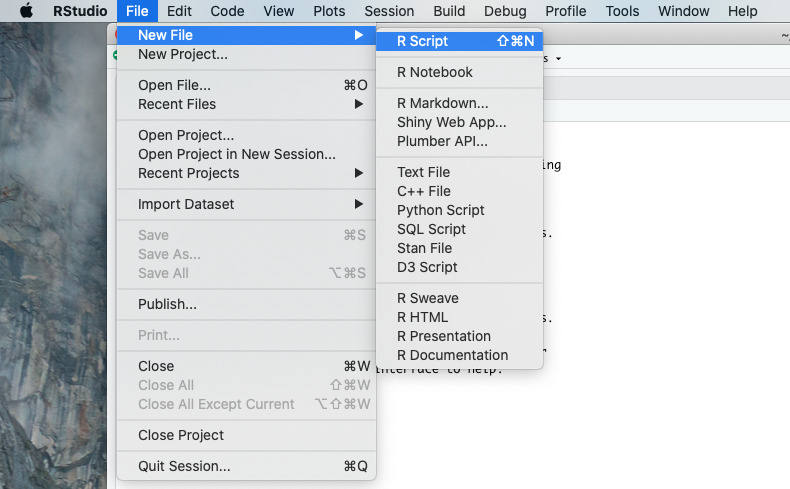
\includegraphics[scale=0.35]{figures/new-script}
\caption{Creating a new script}
\end{figure}

\end{frame}

\begin{frame}{Editor}
\protect\hypertarget{editor}{}

\begin{itemize}
\item
  R opens scripts in the editor pane
\item
  This is where you should write your code
\item
  In the editor you can modify, rerun and save your code at any time
\end{itemize}

\end{frame}

\begin{frame}{Rstudio Panes}
\protect\hypertarget{rstudio-panes}{}

\begin{figure}
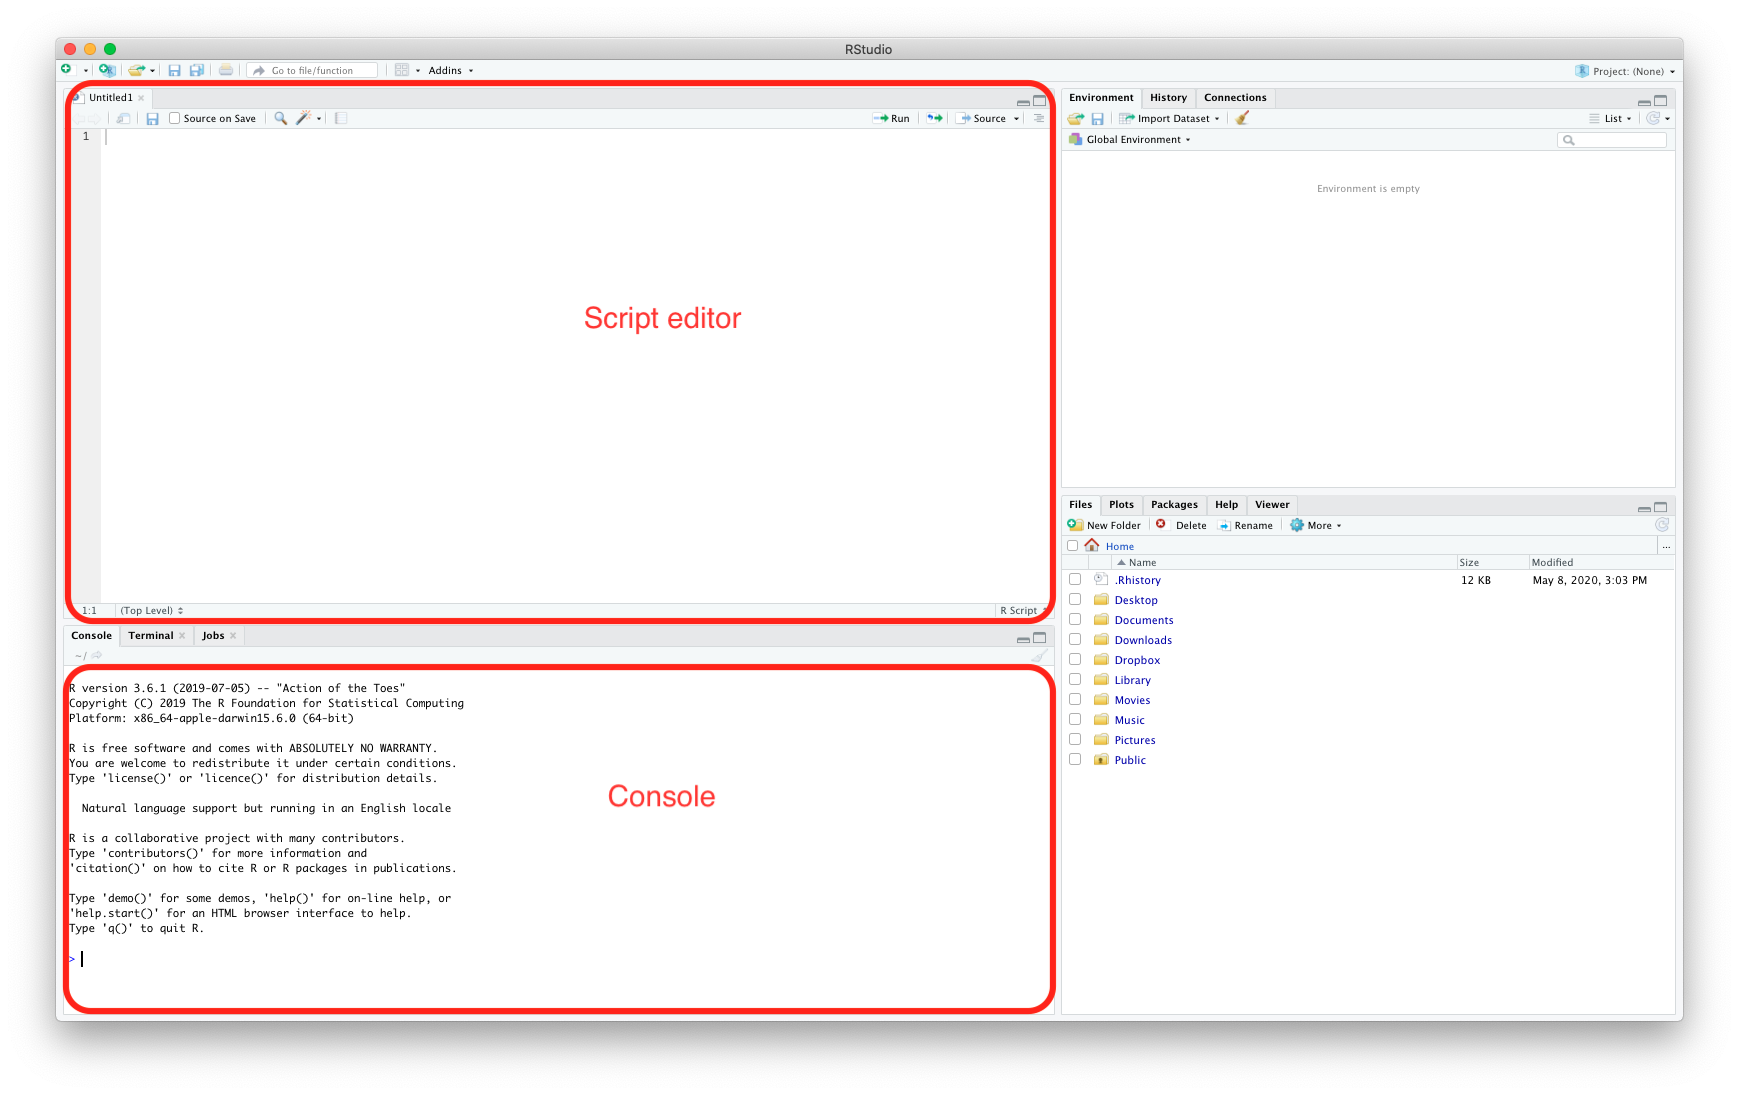
\includegraphics[scale=0.18]{figures/panes}
\caption{R studio's console and editor}
\end{figure}

\end{frame}

\begin{frame}{Some useful shortcuts}
\protect\hypertarget{some-useful-shortcuts}{}

\begin{itemize}
\item
  New script: Cmd/Ctrl + Shift + N
\item
  Save the script: Cmd/Ctrl + S
\item
  Send code from the script to the console:

  \begin{itemize}
  \item
    Cmd/Ctrl + Enter (current line or current selection)
  \item
    Cmd/Ctrl + Shift + S (entire script)
  \end{itemize}
\end{itemize}

\end{frame}

\begin{frame}[fragile]{The assignment operator}
\protect\hypertarget{the-assignment-operator}{}

To store values in R's memory you need to assign them to objects. You
can use the equal sign (\texttt{=}) or the assignment operator
(\texttt{\textless{}-}):

\begin{Shaded}
\begin{Highlighting}[]
\NormalTok{x <-}\StringTok{ }\DecValTok{5}
\NormalTok{x}
\end{Highlighting}
\end{Shaded}

\begin{verbatim}
## [1] 5
\end{verbatim}

\end{frame}

\begin{frame}{The assignment operator}
\protect\hypertarget{the-assignment-operator-1}{}

\begin{itemize}
\item
  The assignment operator is a better option
\item
  The equal sign should be reserved to provide arguments to functions
\item
  Rstudio's shortcut to the assignment operator is ``Alt/Option'' +
  ``\(-\)''
\end{itemize}

\end{frame}

\begin{frame}{The assignment operator}
\protect\hypertarget{the-assignment-operator-2}{}


\includegraphics[scale=.22]{figures/meme}

\end{frame}

\begin{frame}[fragile]{The assignment operator}
\protect\hypertarget{the-assignment-operator-3}{}

Values stored in objects can be used in calculations:

\begin{Shaded}
\begin{Highlighting}[]
\NormalTok{y <-}\StringTok{ }\KeywordTok{log}\NormalTok{(x) }\OperatorTok{+}\StringTok{ }\KeywordTok{exp}\NormalTok{(}\DecValTok{2}\NormalTok{) }
\NormalTok{x }\OperatorTok{+}\StringTok{ }\DecValTok{2} \OperatorTok{*}\StringTok{ }\NormalTok{y}
\end{Highlighting}
\end{Shaded}

\begin{verbatim}
## [1] 22.99699
\end{verbatim}

\end{frame}

\begin{frame}{The assignment operator}
\protect\hypertarget{the-assignment-operator-4}{}

Stored objects are visible in the upper-right pane, under the
``Environment'' tab:

\begin{figure}
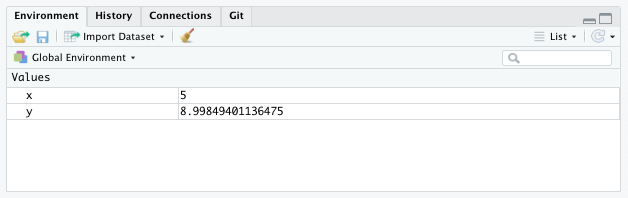
\includegraphics[scale=.45]{figures/objects}
\caption{Our session's global envoronment}
\end{figure}

\end{frame}

\begin{frame}{Workflow}
\protect\hypertarget{workflow}{}

Our workflow so far:

\begin{itemize}
\item
  Write code in the editor
\item
  Send code to the console
\item
  The code is exectued and the results are printed in the console
\item
  The objects we created are listed in the environment tab
\end{itemize}

\end{frame}

\begin{frame}{Workflow}
\protect\hypertarget{workflow-1}{}

\begin{figure}
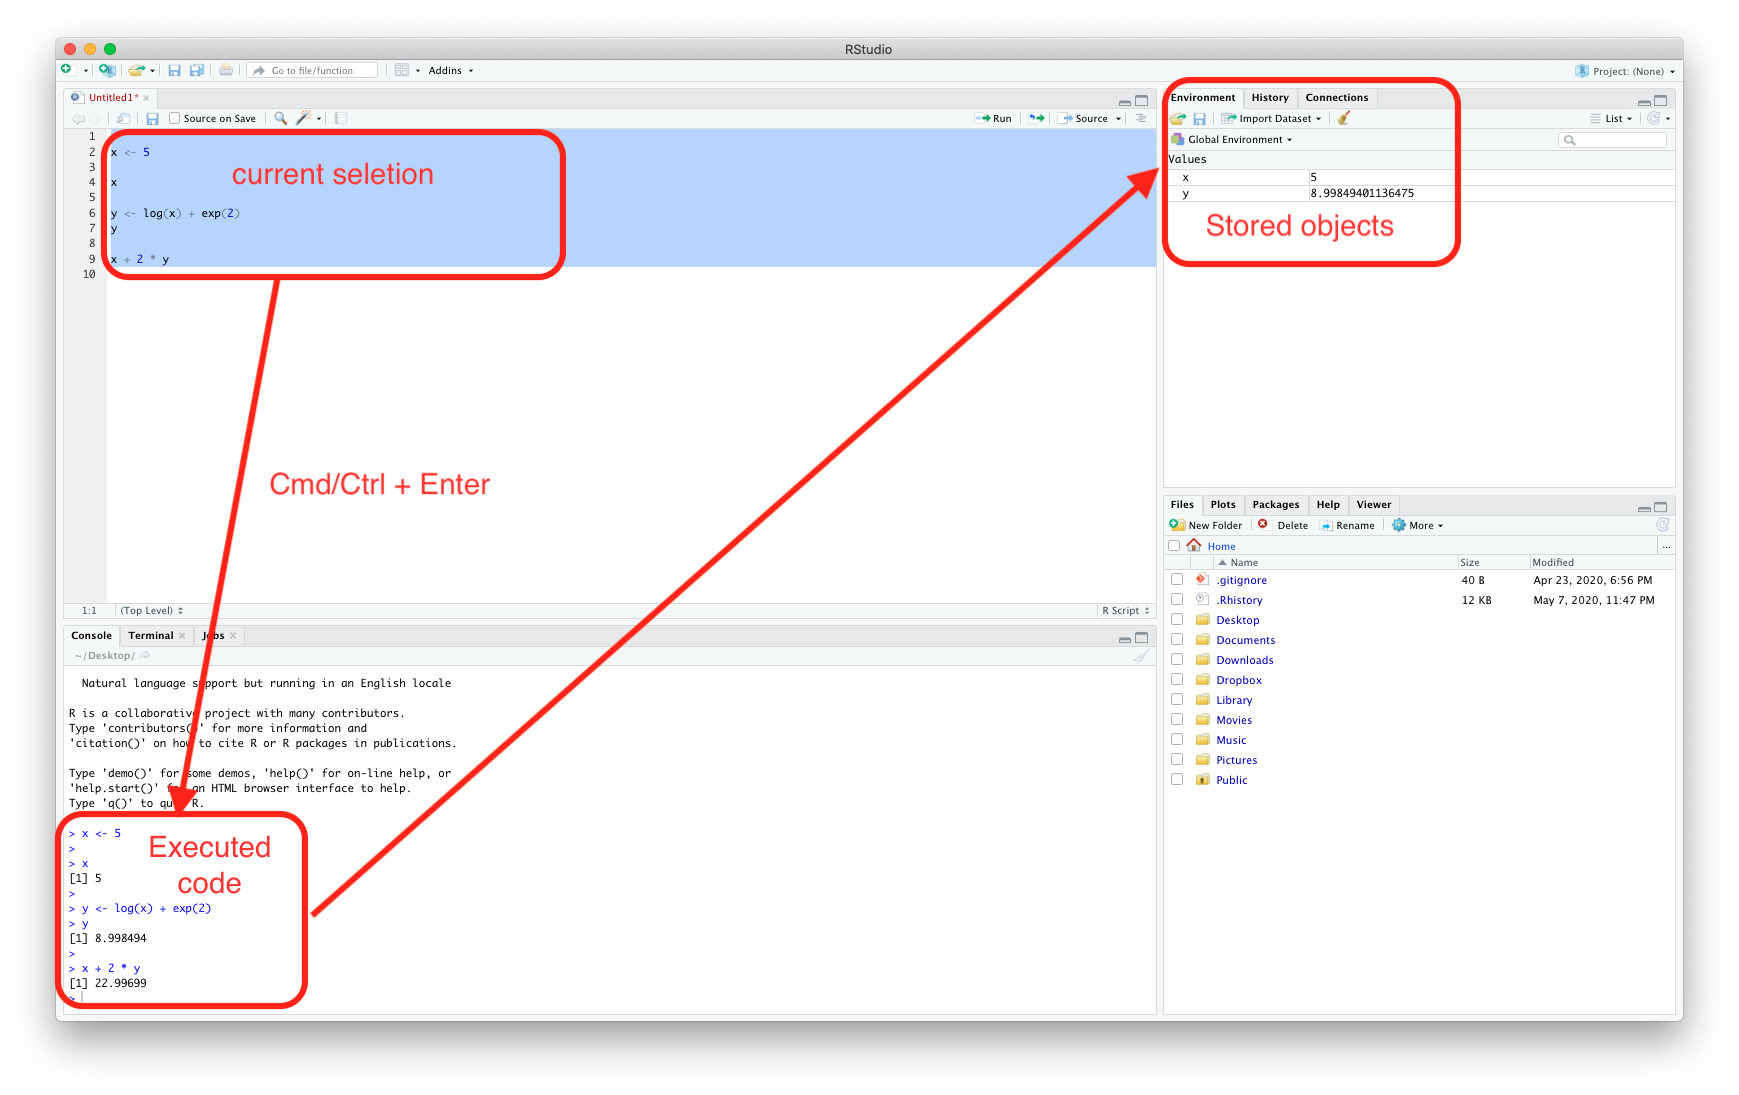
\includegraphics[scale=0.18]{figures/wf}
\caption{Workflow}
\end{figure}

\end{frame}

\begin{frame}[fragile]{Commenting}
\protect\hypertarget{commenting}{}

\begin{itemize}
\item
  We can make comments in our code using \texttt{\#}
\item
  Lines starting with \texttt{\#} are printed in the console but are not
  executed
\end{itemize}

\end{frame}

\begin{frame}[fragile]{Commenting}
\protect\hypertarget{commenting-1}{}

\begin{Shaded}
\begin{Highlighting}[]
\CommentTok{#===================================================}
\CommentTok{# Intro to R programming - Lecture 0}
\CommentTok{#===================================================}

\CommentTok{# Lets store the value "5" in an object called x}
\NormalTok{x <-}\StringTok{ }\DecValTok{5} 

\CommentTok{# Now let's print x}
\NormalTok{x}
\end{Highlighting}
\end{Shaded}

\begin{verbatim}
## [1] 5
\end{verbatim}

\end{frame}

\begin{frame}{Saving scripts}
\protect\hypertarget{saving-scripts}{}

Since we already edited our script, let's save it:

\begin{figure}
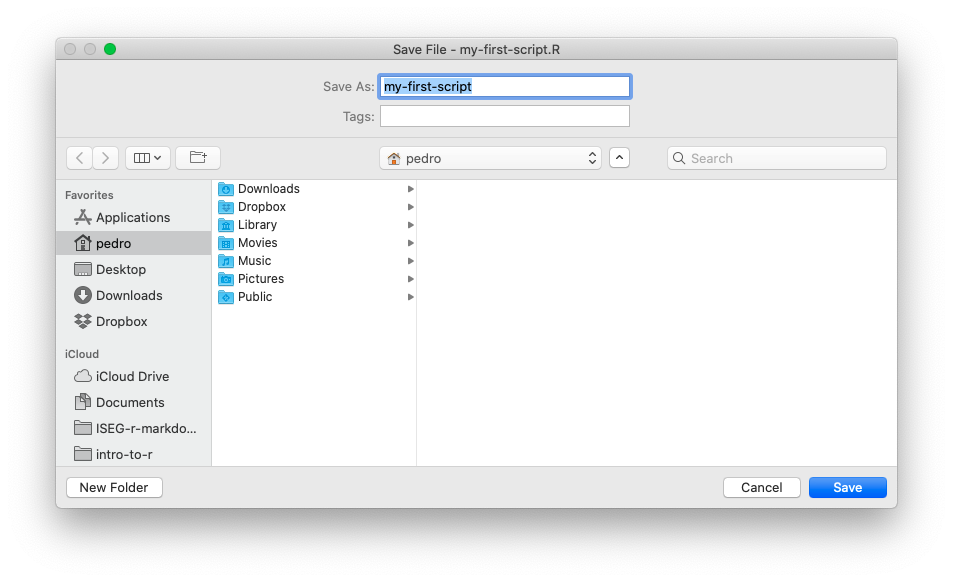
\includegraphics[scale=0.32]{figures/save}
\caption{Saving a script}
\end{figure}

\end{frame}

\begin{frame}{Saving scripts}
\protect\hypertarget{saving-scripts-1}{}

\begin{figure}
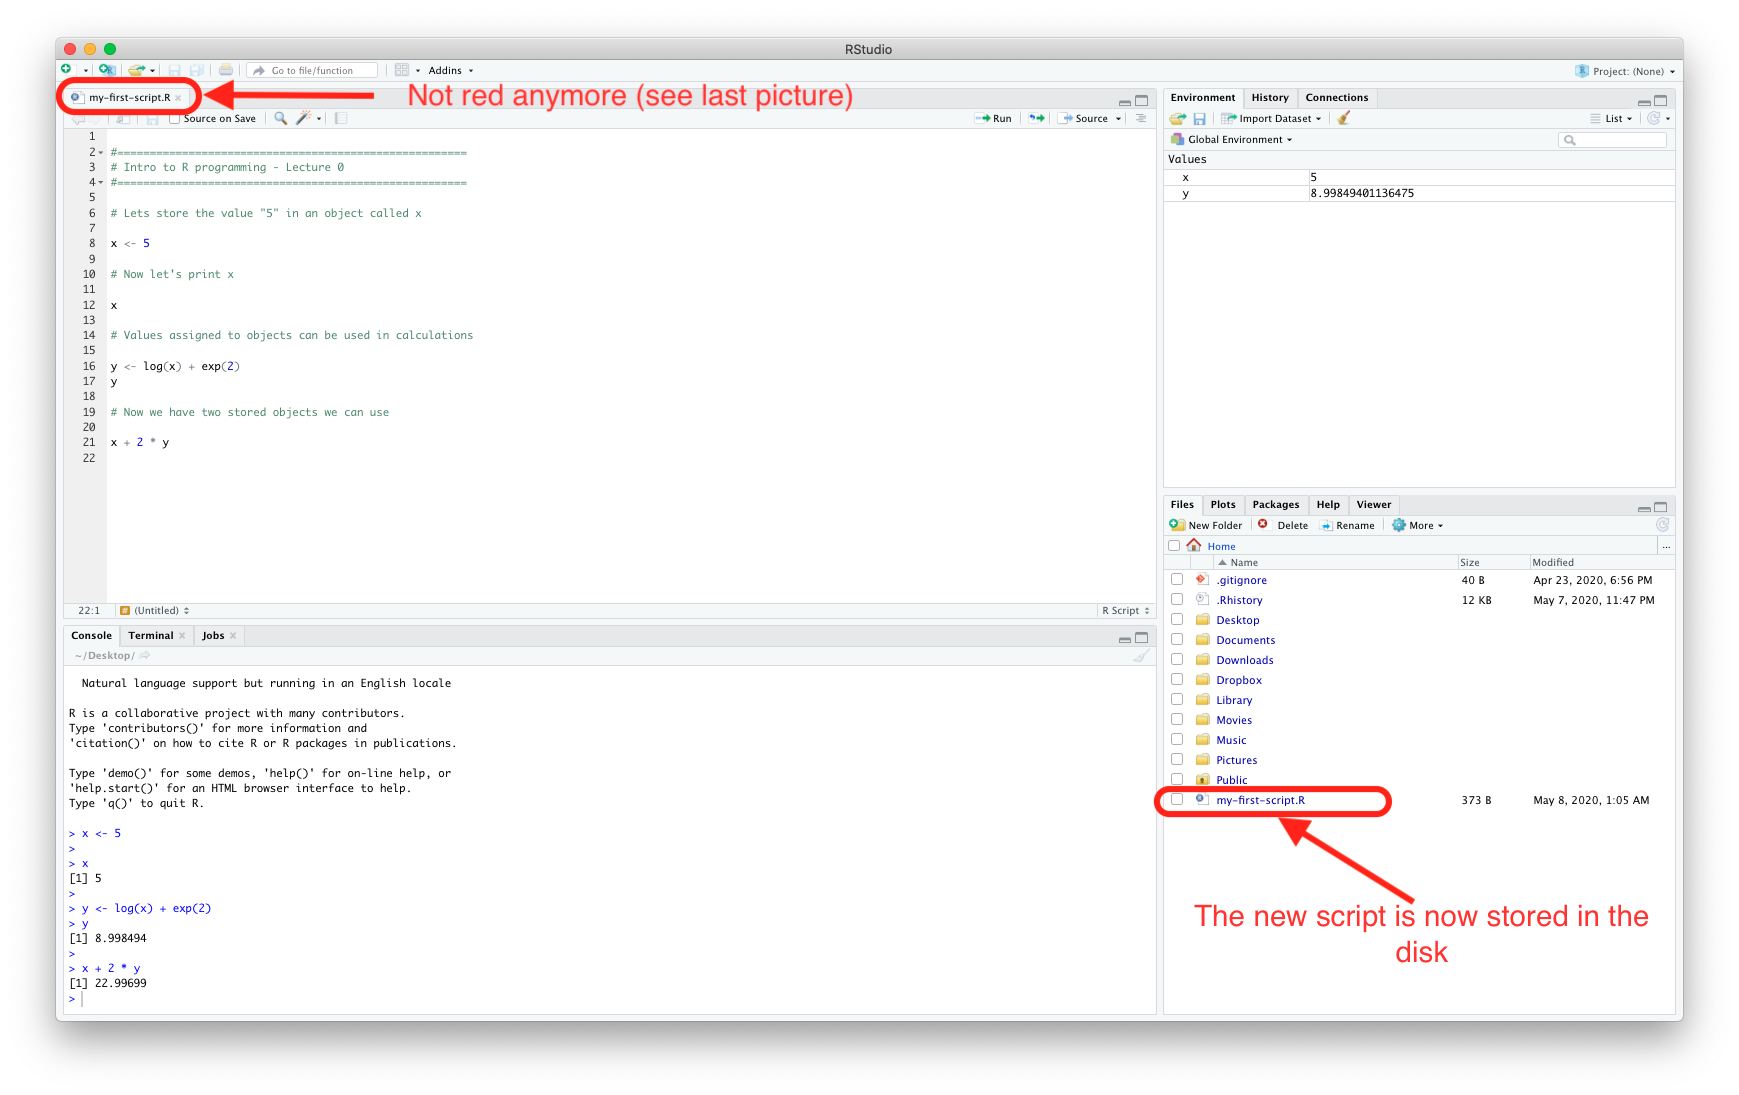
\includegraphics[scale=0.18]{figures/saved}
\caption{The script is now saved}
\end{figure}

\end{frame}

\begin{frame}{Naming Objects}
\protect\hypertarget{naming-objects}{}

\begin{itemize}
\item
  Object names must start with a letter and can only contain letters,
  numbers, underscores and dots
\item
  Ideally, one should follow a convention
\item
  Object names should to be short, descriptive and consistent
\end{itemize}

\end{frame}

\begin{frame}[fragile]{Case matters}
\protect\hypertarget{case-matters}{}

\begin{Shaded}
\begin{Highlighting}[]
\NormalTok{r_rocks <-}\StringTok{ }\DecValTok{2} 
\NormalTok{r_rocks}
\end{Highlighting}
\end{Shaded}

\begin{verbatim}
## [1] 2
\end{verbatim}

\begin{Shaded}
\begin{Highlighting}[]
\NormalTok{r_Rocks}
\end{Highlighting}
\end{Shaded}

\texttt{\#\#\ Error:\ object\ \textquotesingle{}r\_Rocks\textquotesingle{}\ not\ found}

\end{frame}

\begin{frame}[fragile]{How to delete objects}
\protect\hypertarget{how-to-delete-objects}{}

To delete stored objects use the \texttt{rm} function:

\begin{Shaded}
\begin{Highlighting}[]
\NormalTok{r_rocks}
\end{Highlighting}
\end{Shaded}

\begin{verbatim}
## [1] 2
\end{verbatim}

\begin{Shaded}
\begin{Highlighting}[]
\KeywordTok{rm}\NormalTok{(r_rocks)}
\end{Highlighting}
\end{Shaded}

\begin{Shaded}
\begin{Highlighting}[]
\NormalTok{r_rocks}
\end{Highlighting}
\end{Shaded}

\texttt{\#\#\ Error:\ object\ \textquotesingle{}r\_rocks\textquotesingle{}\ not\ found}

\end{frame}

\begin{frame}[fragile]{How to delete objects}
\protect\hypertarget{how-to-delete-objects-1}{}

You can input as many objects as you want to \texttt{rm()}:

\begin{Shaded}
\begin{Highlighting}[]
\KeywordTok{rm}\NormalTok{(x, y)}
\end{Highlighting}
\end{Shaded}

To remove all stored objects all once, use the following command:

\begin{Shaded}
\begin{Highlighting}[]
\KeywordTok{rm}\NormalTok{(}\DataTypeTok{list =} \KeywordTok{ls}\NormalTok{())}
\end{Highlighting}
\end{Shaded}

\end{frame}

\begin{frame}[fragile]{Overwritting stored values}
\protect\hypertarget{overwritting-stored-values}{}

\begin{Shaded}
\begin{Highlighting}[]
\NormalTok{x <-}\StringTok{ }\DecValTok{-5}
\NormalTok{x}
\end{Highlighting}
\end{Shaded}

\begin{verbatim}
## [1] -5
\end{verbatim}

\begin{Shaded}
\begin{Highlighting}[]
\NormalTok{x <-}\StringTok{ }\NormalTok{x }\OperatorTok{+}\StringTok{ }\DecValTok{1} 
\NormalTok{x}
\end{Highlighting}
\end{Shaded}

\begin{verbatim}
## [1] -4
\end{verbatim}

\begin{Shaded}
\begin{Highlighting}[]
\NormalTok{x <-}\StringTok{ }\KeywordTok{round}\NormalTok{(}\KeywordTok{log}\NormalTok{(}\DecValTok{3}\NormalTok{)}\OperatorTok{/}\DecValTok{2}\NormalTok{, }\DataTypeTok{digits =} \DecValTok{2}\NormalTok{)}
\NormalTok{x}
\end{Highlighting}
\end{Shaded}

\begin{verbatim}
## [1] 0.55
\end{verbatim}

\end{frame}

\begin{frame}[fragile]{Working directory}
\protect\hypertarget{working-directory}{}

An R session always has an associated working directory. R will use the
working directory by default to:

\begin{itemize}
\item
  Search for files
\item
  Save files
\item
  Save outputs (tables, plots, etc)
\end{itemize}

To check your workig directory:

\begin{Shaded}
\begin{Highlighting}[]
\KeywordTok{getwd}\NormalTok{()}
\end{Highlighting}
\end{Shaded}

\end{frame}

\begin{frame}{Setting the working directory}
\protect\hypertarget{setting-the-working-directory}{}

You can change your working directory using RStudio's menus:

\begin{figure}
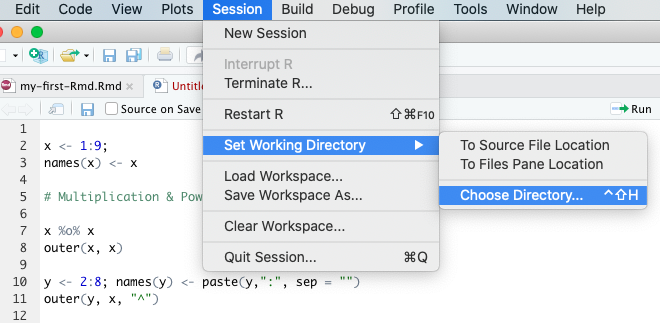
\includegraphics[scale = .40]{figures/wd}
\caption{Setting the working directory}
\end{figure}

\end{frame}

\begin{frame}[fragile]{Setting and setting the working directory}
\protect\hypertarget{setting-and-setting-the-working-directory}{}

You can also change the working directory in R's console:

\begin{Shaded}
\begin{Highlighting}[]
\KeywordTok{setwd}\NormalTok{(}\StringTok{"/Users/pedro/Documents/intro-to-r"}\NormalTok{)}
\end{Highlighting}
\end{Shaded}

The problem with absolute paths is that they will only exist on your
computer. Solution:

\begin{itemize}
\tightlist
\item
  Rstudio projects
\end{itemize}

\end{frame}

\begin{frame}{Your first Rstudio project}
\protect\hypertarget{your-first-rstudio-project}{}

\begin{figure}
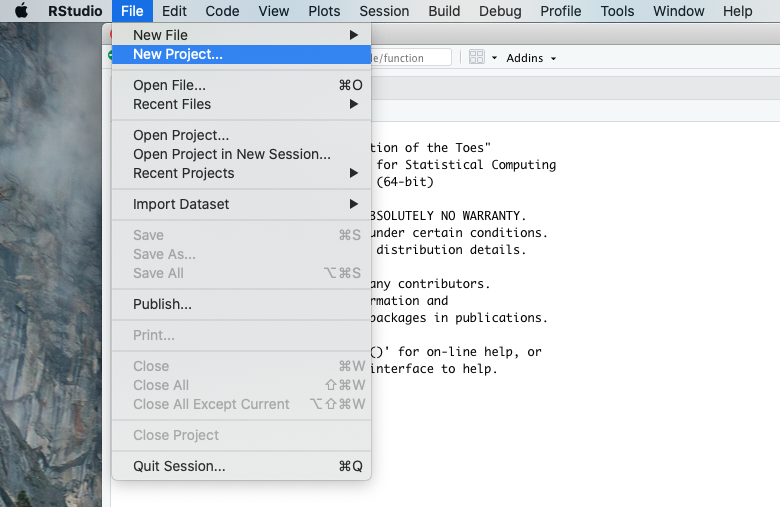
\includegraphics[scale=0.35]{figures/new-project-1}
\end{figure}

\end{frame}

\begin{frame}{Your first Rstudio project}
\protect\hypertarget{your-first-rstudio-project-1}{}

\begin{figure}
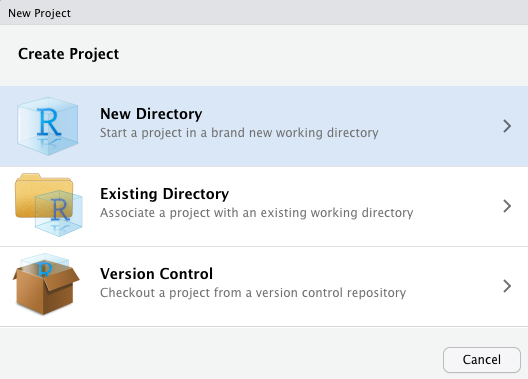
\includegraphics[scale=0.43]{figures/new-project-2}
\end{figure}

\end{frame}

\begin{frame}{Your first Rstudio project}
\protect\hypertarget{your-first-rstudio-project-2}{}

\begin{figure}
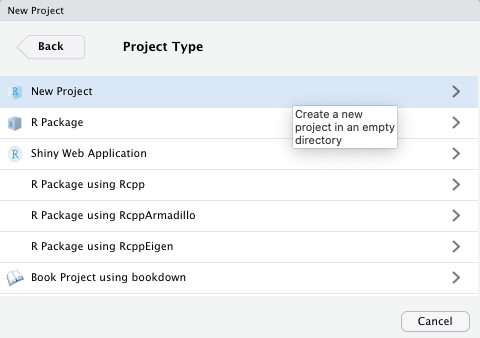
\includegraphics[scale=0.43]{figures/new-project-3}
\end{figure}

\end{frame}

\begin{frame}{Your first Rstudio project}
\protect\hypertarget{your-first-rstudio-project-3}{}

\begin{figure}
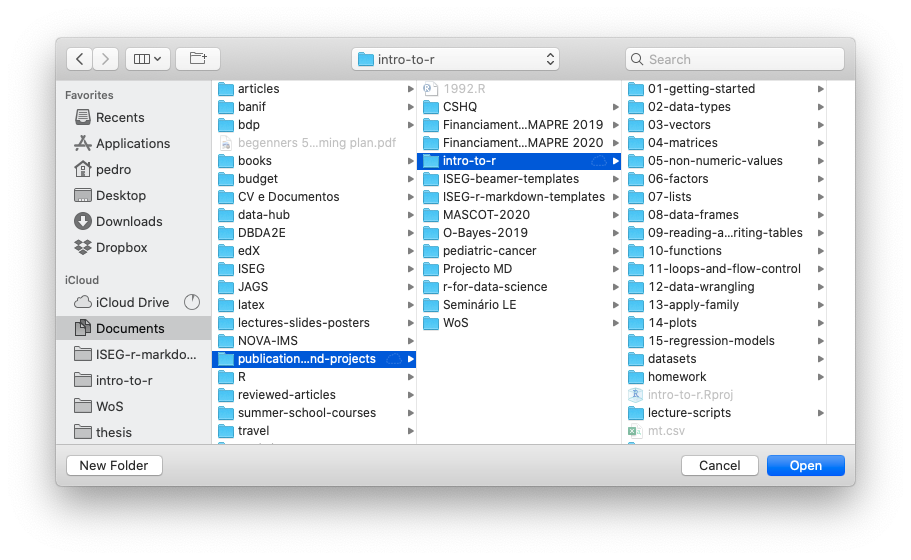
\includegraphics[scale=0.43]{figures/new-project-4}
\end{figure}

\end{frame}

\begin{frame}{Your first Rstudio project}
\protect\hypertarget{your-first-rstudio-project-4}{}

\begin{figure}
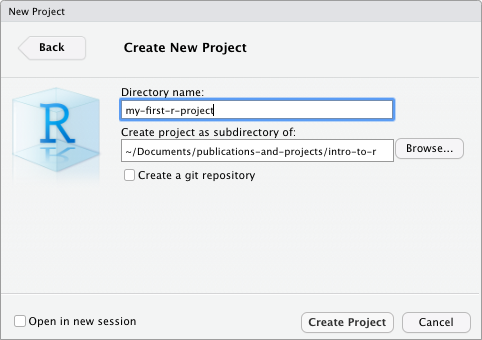
\includegraphics[scale=0.33]{figures/new-project-5}
\end{figure}

\end{frame}

\begin{frame}{Your first Rstudio project}
\protect\hypertarget{your-first-rstudio-project-5}{}

\begin{figure}
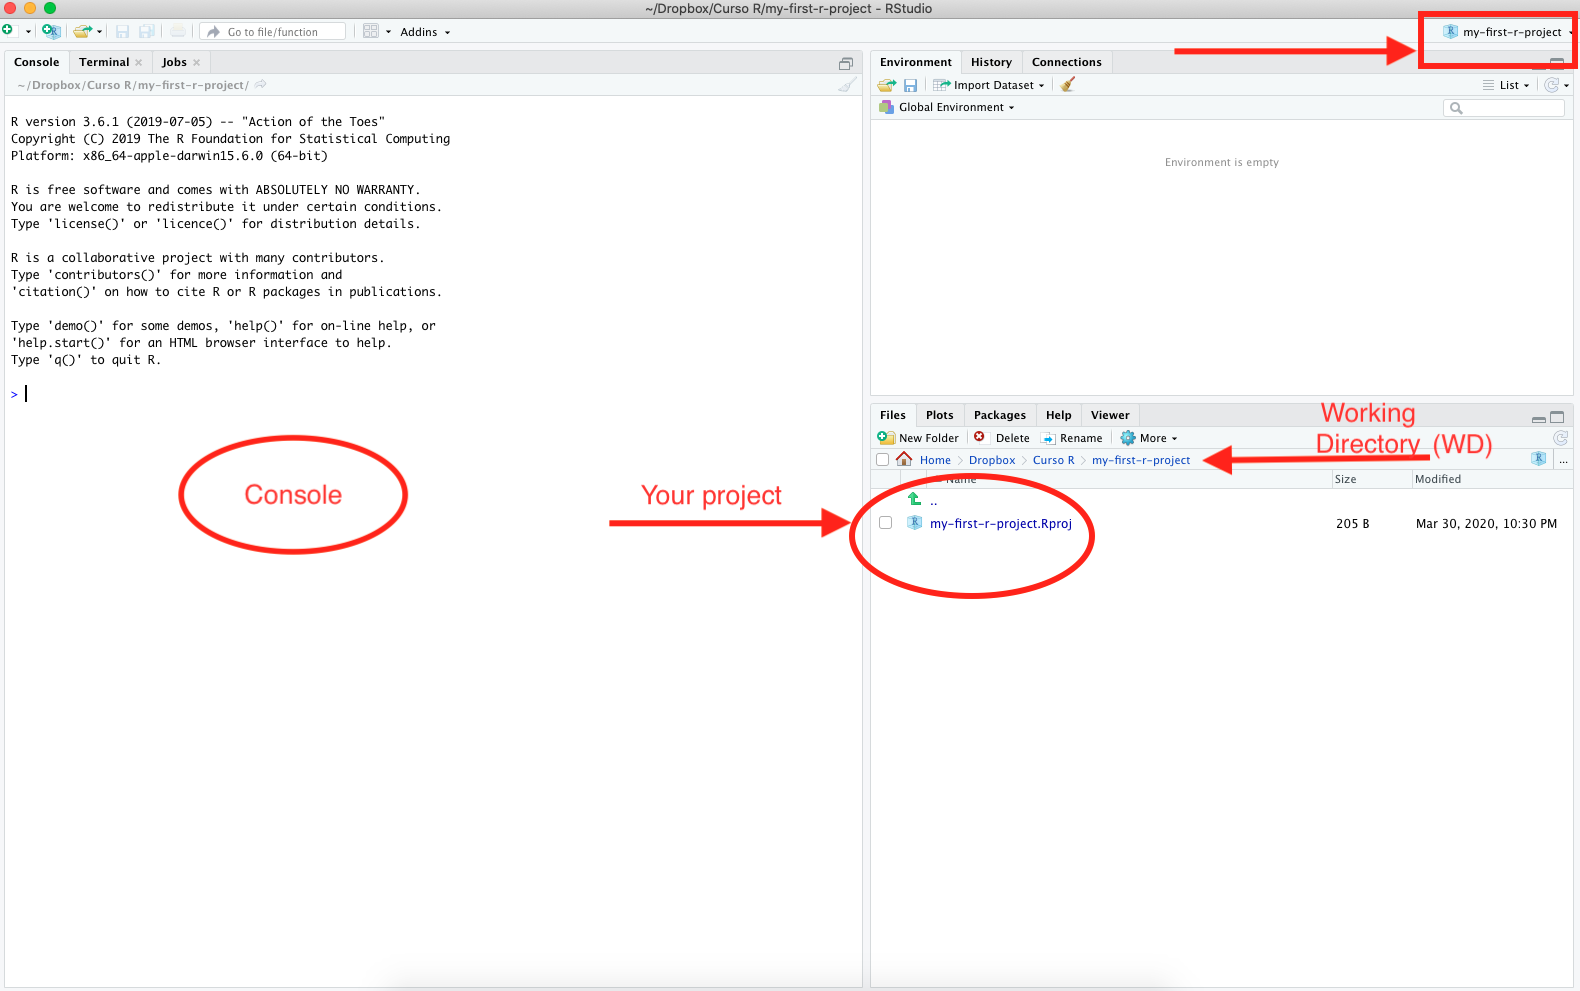
\includegraphics[scale=0.19]{figures/environment}
\end{figure}

\end{frame}

\begin{frame}[fragile]{Advantages of Rstudio projects}
\protect\hypertarget{advantages-of-rstudio-projects}{}

\begin{itemize}
\item
  Rstudio projects are self-contained.
\item
  They put together all the files that are relevant for a particular
  project (article, book, research project) in the same folder
\item
  The project's working directory always points to that folder by
  default
\item
  Rstudio projects can be moved around on your computer or onto other
  computers and will still ``just work''. No directory changes are
  needed.
\item
  If you need to create additional folders or start moving around parts
  of you project around dont use the \texttt{setwd} function. It is
  safer to reference the full path.
\end{itemize}

\end{frame}

\begin{frame}{Packages}
\protect\hypertarget{packages}{}

\begin{itemize}
\item
  The more specialized functions are distributed on packages
\item
  Packages are developed by the R core team and also by the community of
  R users
\item
  You can develop your own packages and make them available to the
  community through \href{https://cran.r-project.org}{CRAN} (The
  Comprehensive R Archive Network)
\end{itemize}

\end{frame}

\begin{frame}[fragile]{Packages}
\protect\hypertarget{packages-1}{}

Later in this course, we will use the \texttt{sqldf} package. Let's
install it:

\begin{Shaded}
\begin{Highlighting}[]
\KeywordTok{install.packages}\NormalTok{(}\StringTok{"sqldf"}\NormalTok{)}
\end{Highlighting}
\end{Shaded}

If you want to use an installed package, you must load it first:

\begin{Shaded}
\begin{Highlighting}[]
\KeywordTok{library}\NormalTok{(}\StringTok{"sqldf"}\NormalTok{)}
\end{Highlighting}
\end{Shaded}

Update an installed package:

\begin{Shaded}
\begin{Highlighting}[]
\KeywordTok{update.packages}\NormalTok{(}\StringTok{"sqldf"}\NormalTok{) }
\end{Highlighting}
\end{Shaded}

\end{frame}

\begin{frame}{Packages}
\protect\hypertarget{packages-2}{}

\begin{itemize}
\item
  It is recommended that you start your scripts by loading the packages
  that will be used
\item
  That way, if you share your code with others (even if that's future
  you), they can easily see what packages they need to install
\end{itemize}

\end{frame}

\begin{frame}[fragile]{Packages}
\protect\hypertarget{packages-3}{}

\begin{itemize}
\item
  Note, however, that you should never include \texttt{install.packages}
  or \texttt{setwd} in a script that you share
\item
  Use \texttt{library} instead
\item
  It is very antisocial to change settings or install software on
  someone else's computer!
\end{itemize}

\end{frame}

\end{document}
